% !TeX spellcheck = es_MX-SpanishMexico
%----------------------------------------------------------------------------------------------------
%                           		  ENTRE LÍNEAS DE TIERRA

% Curso: Arqueología Bíblica
% Módulo 1: Introducción, Definiciones y Conceptos
% Elabora: Rodrigo Gerardo Trejo Arriaga

%----------------------------------------------------------------------------------------------------

% FORMATO DEL DOCUMENTO


\documentclass[11pt]{article} % Letra estandar

\usepackage[utf8]{inputenc}

%\usepackage{tgadventor}
%\renewcommand{\familydefault}{\sfdefault}

\usepackage[light,math]{iwona}

\usepackage[T1]{fontenc}


\usepackage[spanish]{babel}
\addto\captionsspanish{\renewcommand{\abstractname}{\large{Introducción}}}

\usepackage[margin=1in,letterpaper]{geometry}

\usepackage{fancyhdr} % Paquete para personalizar encabezado y pie de página
\pagestyle{fancy} % Establece que personalizaremos el pie de pagina y el encabezado
\setlength{\headheight}{13.59999pt} % Establece la altura del encabezado
\fancyhead[R]{\textcolor{darkBlue}{Teoría de la Computación}} % Encabezado derecho
\fancyhead[L]{\textit{\textcolor{darkBlue}{Escuela Superior de Cómputo}}} % Encabezado izquierdo
\fancyfoot[L]{\textit{\textcolor{darkBlue}{Práctica 7}}} % Pie de página izquierdo 
\fancyfoot[R]{\textcolor{darkBlue}{\thepage}} % Pie de página  derecho
\fancyfoot[C]{} % Elimina la nueración central de páginas en el pie de página
\renewcommand{\headrulewidth}{0.5pt} % Grosor de la linea de encabezado
\renewcommand{\footrulewidth}{0.5pt} % Grosor de la linea de pie de página

\usepackage{enumitem}

\usepackage{changepage}

\usepackage{graphicx}

\usepackage{tabularx}

\setlength{\parskip}{8pt}

\usepackage{xcolor}
\definecolor{darkBlue}{rgb}{0,0,0.31}
%\definecolor{darkBlue}{rgb}{0,0,0.5}
\definecolor{munsell}{rgb}{0.0, 0.5, 0.69}
\definecolor{indigo}{rgb}{0.0, 0.25, 0.42}
\renewcommand{\footrulewidth}{2pt}
\renewcommand{\footrule}{\hbox to\headwidth{\color{darkBlue}\leaders\hrule height \footrulewidth\hfill}}

\usepackage{colortbl}

\usepackage{titlesec}
\titleformat{\section}
{\normalfont\Large\bfseries\color{darkBlue}}{\thesection.}{1em}{}

\usepackage{tabularx}

\usepackage{textcomp}

\usepackage{titling}

\usepackage{apacite}

\usepackage{amsmath}
\bibliographystyle{apacite}

%\usepackage{natbib}
%\setlength{\bibsep}{6pt}

\usepackage{setspace}

\usepackage{listings}


% Define tus propios colores en tonos de azul
\definecolor{codeblue}{rgb}{0.25,0.5,0.5}
\definecolor{backcolour}{rgb}{0.95,0.95,0.92}
\definecolor{commentblue}{rgb}{0.3,0.3,0.6}
\definecolor{keywordblue}{rgb}{0.2,0.2,0.7}
\definecolor{stringblue}{rgb}{0.15,0.2,0.9}

\lstdefinestyle{bluepythonstyle}{
	language=Python,
	basicstyle=\ttfamily\small,
	commentstyle=\color{commentblue},
	keywordstyle=\color{keywordblue},
	numberstyle=\tiny\color{codeblue},
	stringstyle=\color{stringblue},
	backgroundcolor=\color{backcolour},
	breaklines=true,
	captionpos=b,
	abovecaptionskip=1\baselineskip,
	showstringspaces=false,
	frame=lines,
	numbers=left,
	xleftmargin=\parindent,
	tabsize=4
}
\lstset{style=bluepythonstyle}



\renewcommand{\thesection}{\Roman{section}}

%----------------------------------------------------------------------------------------------------
% CUERPO DEL DOCUMENTO

\begin{document}
	
	\begin{titlepage}
		\centering
		{
\includegraphics[width=0.25\textwidth]{descarga}\par}
		\vspace{0.5cm}
		{\bfseries\huge Escuela Superior de Cómputo \par}
		\vspace{0.7cm}
		{\scshape\LARGE Teoría de la Computación \par}
		\vspace{0.3cm}
		\vspace{3.1cm}
		{\scshape \Huge \textbf{Práctica 7:}  \par}
		\vspace{0.03cm}
		{{\LARGE \textit{LENGUAJES LIBRES DE CONTEXTO - PALÍNDROMOS}} \par}
		%\vfill
		\vspace{3.5cm}
		{\Large Autor: \par}
		{\Large Rodrigo Gerardo Trejo Arriaga \par}
		%\vfill
		\vspace{3cm}
		{\Large Diciembre 2023 \par}
	\end{titlepage}
	
	\begin{center}
		\vspace*{0.1cm}
		{\huge \textcolor{darkBlue}{\textbf{Práctica 7:}} \par}
		
		{\Large \textcolor{darkBlue}{\textbf{\textit{LENGUAJES LIBRES DE CONTEXTO - PALÍNDROMOS}}}}
	\end{center}
	
	
	\section{Introducción}
	Un \textbf{lenguaje libre de contexto} es un tipo de lenguaje formal que tiene gran importancia en la teoría de la computación y la teoría de autómatas. Los lenguajes libres de contexto son generados por gramáticas libres de contexto y son reconocidos por autómatas de pila [1].
	
	\section{Definición [1]}
	Una gramática libre de contexto (GLC) se define como una cuádrupla \(G = (V, \Sigma, R, S)\), donde:
	\begin{itemize}
		\item \(V\) es un conjunto finito de variables (también llamadas símbolos no terminales).
		\item \(\Sigma\) es un conjunto finito de símbolos terminales, disjunto de \(V\).
		\item \(R\) es un conjunto finito de reglas de producción, cada una de la forma \(A \rightarrow \beta\), donde \(A \in V\) y \(\beta \in (V \cup \Sigma)^*\).
		\item \(S \in V\) es el símbolo inicial.
	\end{itemize}
	
	\section{Características [2]}
	\begin{enumerate}
		\item \textbf{Independencia del Contexto:} En una GLC, la producción a aplicar depende solo del símbolo no terminal a reemplazar, y no del contexto (símbolos adyacentes) en el que aparece.
		\item \textbf{Jerarquía de Chomsky:} Los lenguajes libres de contexto se sitúan en el segundo nivel de la Jerarquía de Chomsky, entre los lenguajes regulares y los lenguajes sensibles al contexto.
		\item \textbf{Autómatas de Pila:} Estos lenguajes pueden ser reconocidos por autómatas de pila, que son máquinas abstractas con capacidad de almacenamiento adicional en forma de pila.
	\end{enumerate}
	
	\section{Ejemplos [2]}
	Un ejemplo clásico de lenguaje libre de contexto es el lenguaje de paréntesis balanceados, definido por la gramática \(G = (\{S\}, \{(, )\}, R, S)\) con \(R = \{S \rightarrow SS, S \rightarrow (S), S \rightarrow \varepsilon\}\).
	
	Los lenguajes libres de contexto son fundamentales en el diseño de lenguajes de programación y en el análisis sintáctico en compiladores.
	
	\section{Palíndromos y Lenguajes Libres de Contexto}
	Un palíndromo es una secuencia de símbolos que se lee igual hacia adelante y hacia atrás. Los lenguajes libres de contexto pueden describir palíndromos de manera eficiente mediante reglas de producción.
	

	La generación de palíndromos utilizando una gramática libre de contexto se basa en la construcción simétrica de la cadena. Por ejemplo, consideremos la gramática \(G = (V, \Sigma, R, S)\) con:
	\begin{itemize}
		\item \(V = \{P\}\)
		\item \(\Sigma = \{0, 1\}\)
		\item \(R = \{ P \rightarrow \varepsilon, P \rightarrow 0, P \rightarrow 1, P \rightarrow 0P0, P \rightarrow 1P1 \}\)
		\item \(S = P\)
	\end{itemize}
	
	\subsection*{Ventajas}
	\begin{enumerate}
		\item \textbf{Estructura Simétrica:} Las reglas de producción permiten construir la cadena de manera simétrica, garantizando la propiedad palindrómica.
		\item \textbf{Flexibilidad:} Los lenguajes libres de contexto pueden generar palíndromos de diferentes longitudes y complejidades.
		\item \textbf{Automatización:} Facilitan la automatización en la generación de palíndromos, especialmente útil en aplicaciones de procesamiento de lenguajes y criptografía.
	\end{enumerate}
	
	\section{Instrucciones}
	Este programa en Python genera palíndromos en un lenguaje binario según una gramática libre de contexto. El usuario puede elegir la longitud del palíndromo o permitir que el programa lo genere automáticamente. La longitud máxima es de 10,000 caracteres.
	
	\subsection*{Gramática Libre de Contexto}
	La gramática se define con las siguientes reglas de producción:
	\begin{enumerate}
		\item \( P \rightarrow \varepsilon \)
		\item \( P \rightarrow 0 \)
		\item \( P \rightarrow 1 \)
		\item \( P \rightarrow 0P0 \)
		\item \( P \rightarrow 1P1 \)
	\end{enumerate}
	
	
	
	\section{Resultados}
	
	
	\begin{figure}[h]
		\centering
		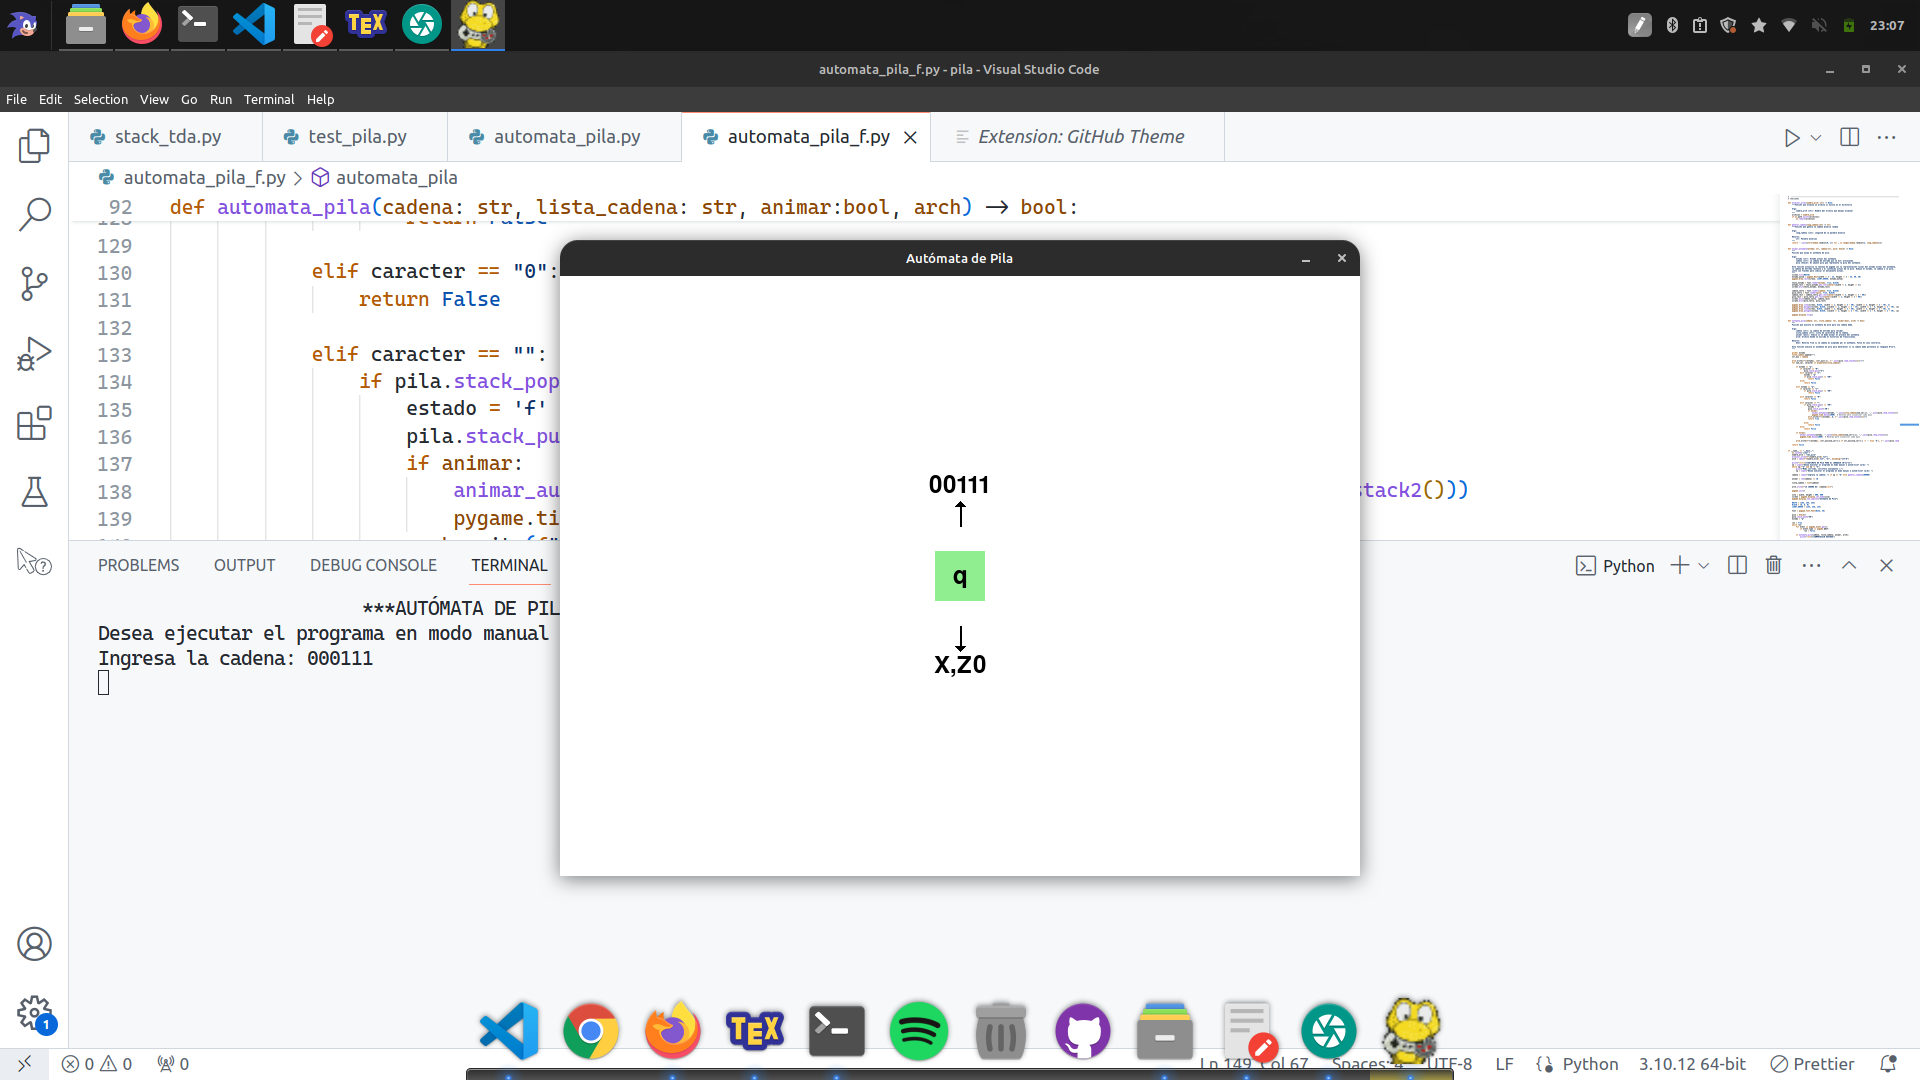
\includegraphics[width=0.8\textwidth]{manual}
		\caption{Modo manual - Longitud par}
	\end{figure}
	
	\begin{figure}[h]
		\centering
		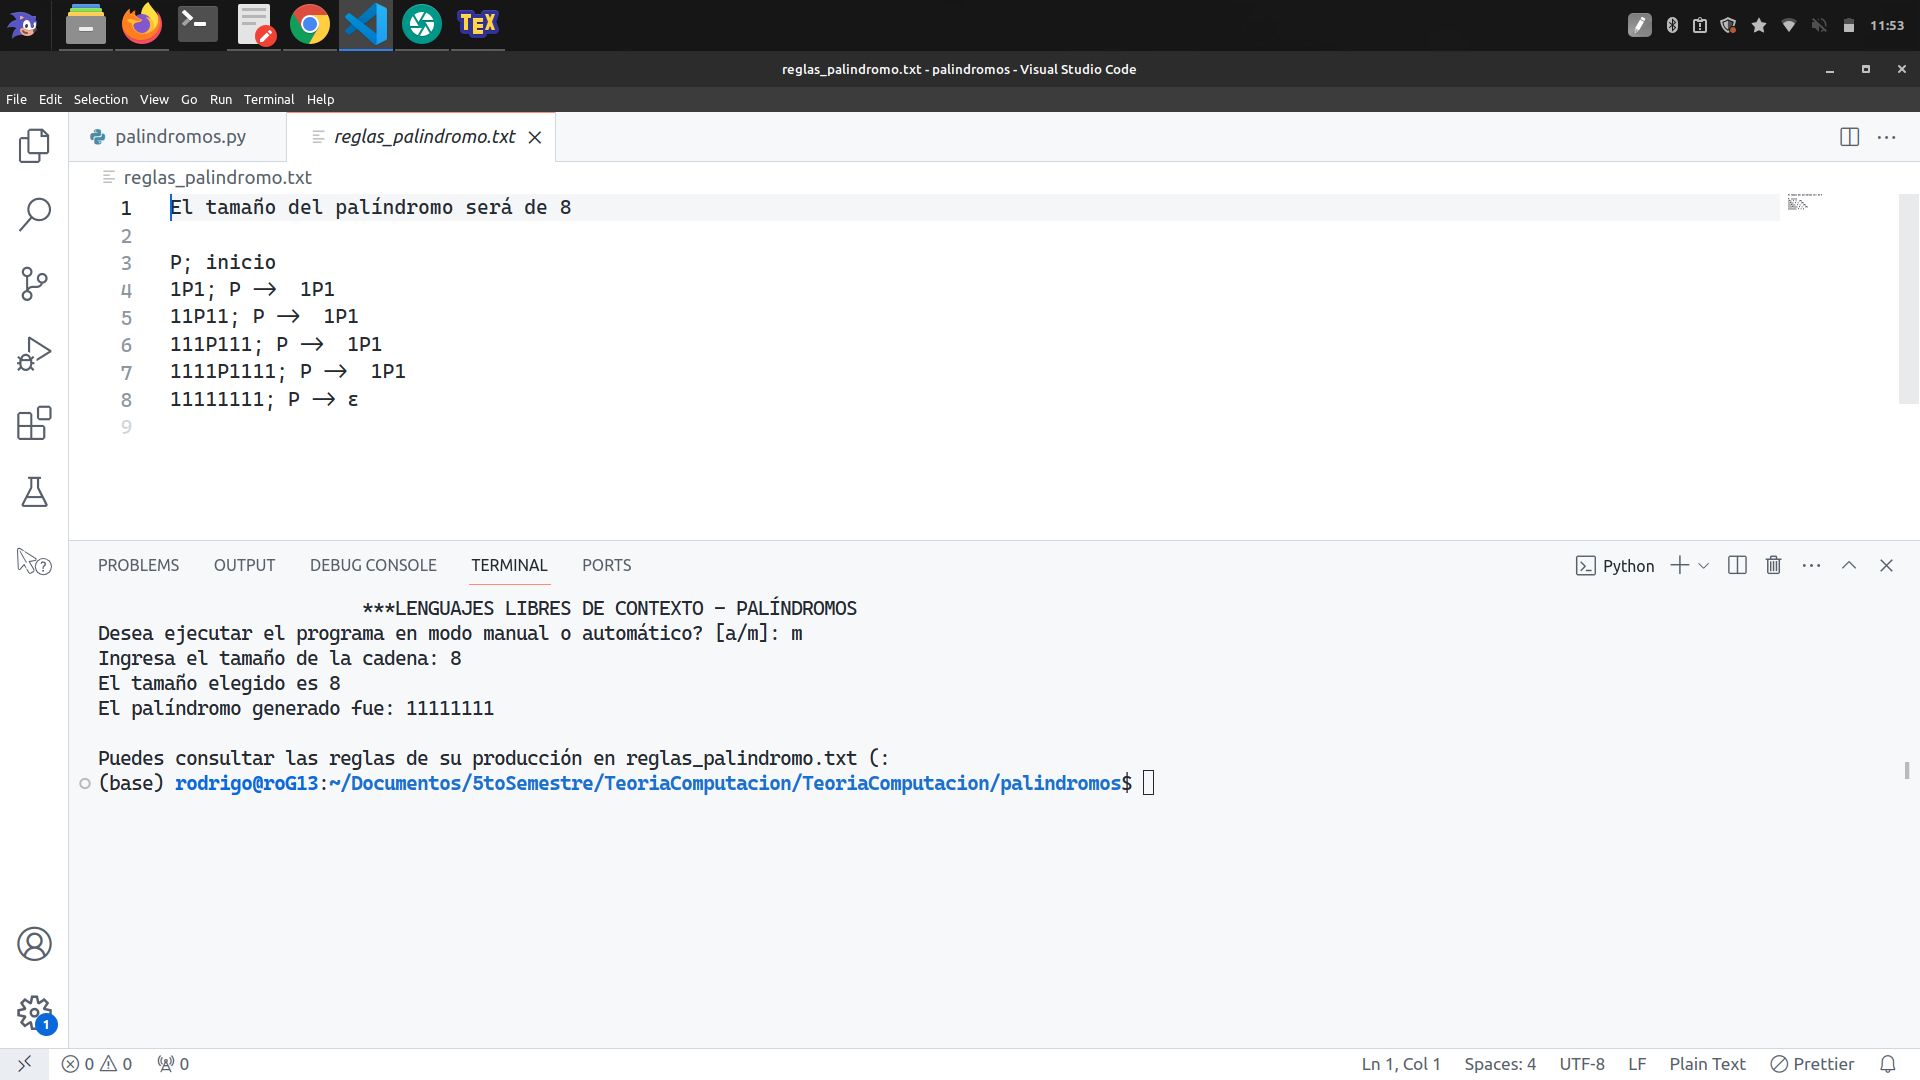
\includegraphics[width=0.8\textwidth]{arch1}
		\caption{Modo manual - Longitud par - Archivo}
	\end{figure}
	
	\newpage
	
	\begin{figure}[h]
		\centering
		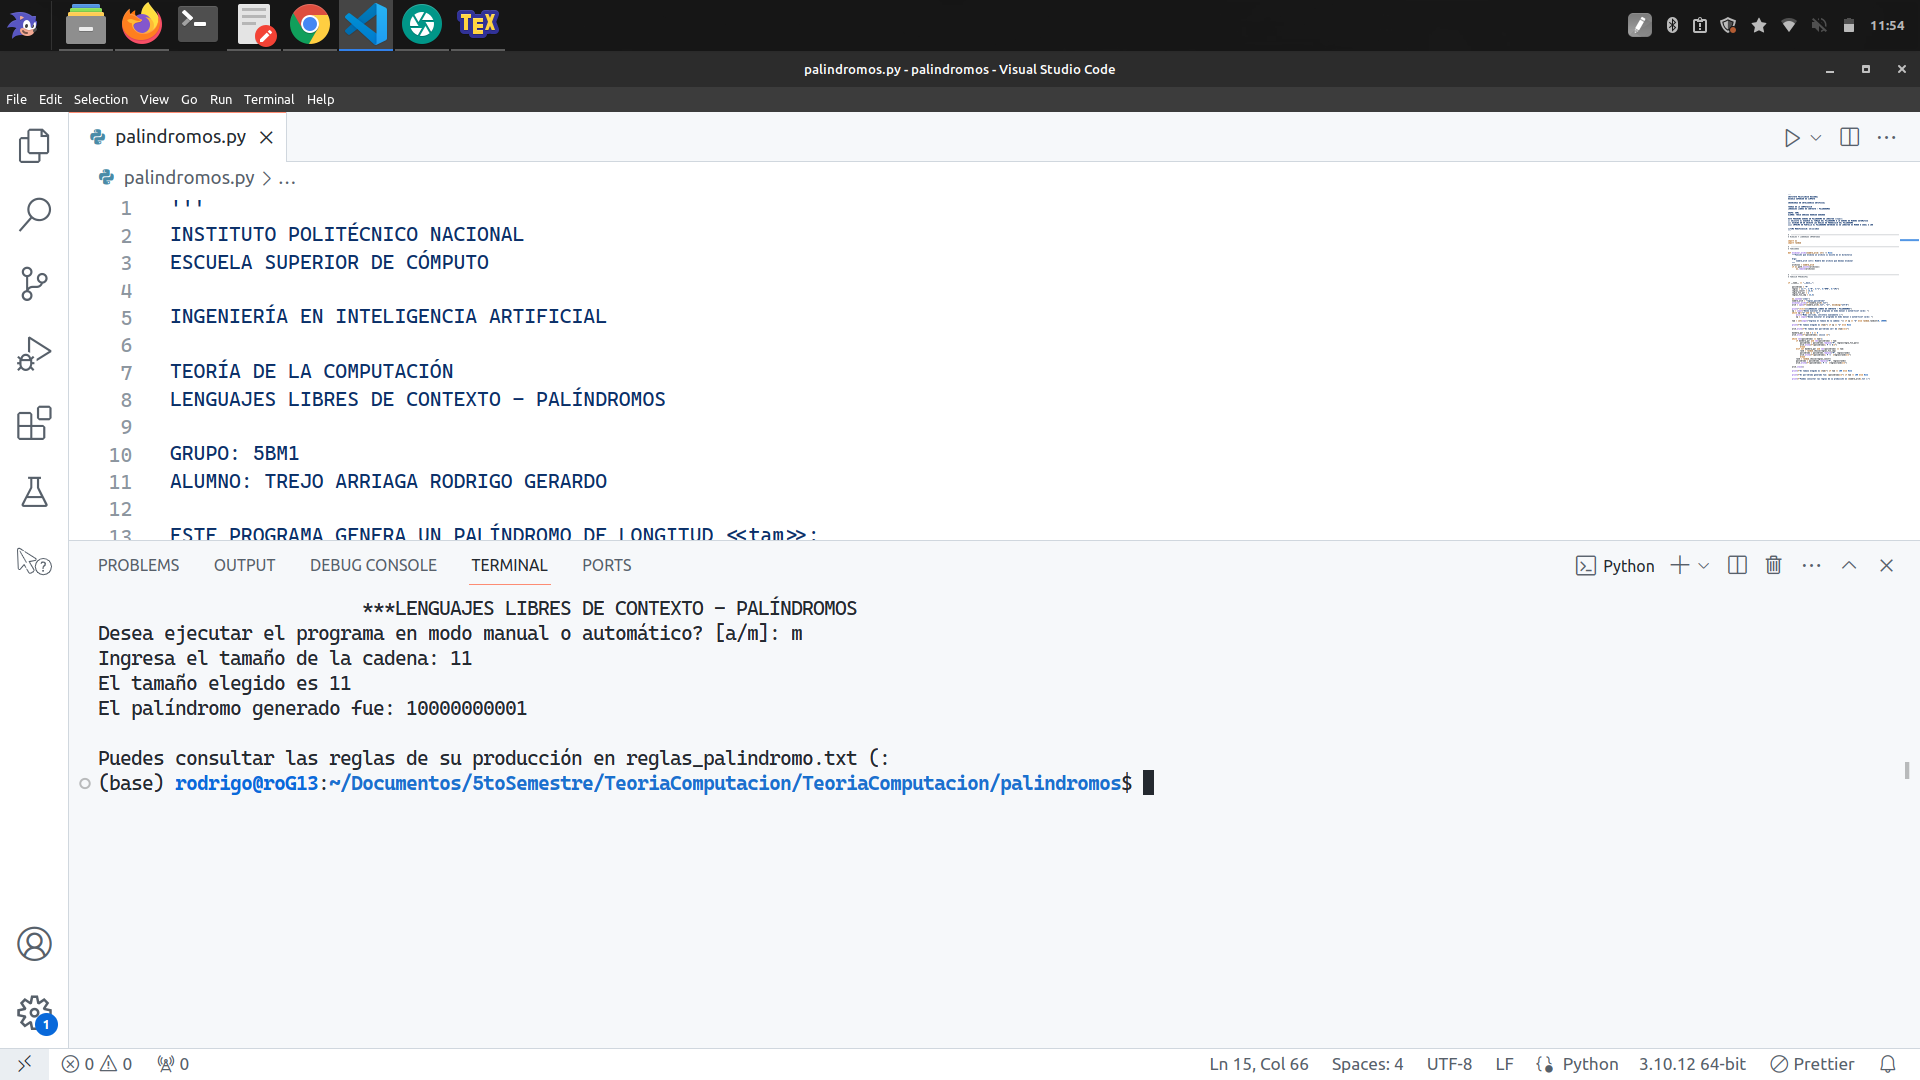
\includegraphics[width=0.8\textwidth]{manual2}
		\caption{Modo manual - Longitud impar}
	\end{figure}
	
	\begin{figure}[h]
		\centering
		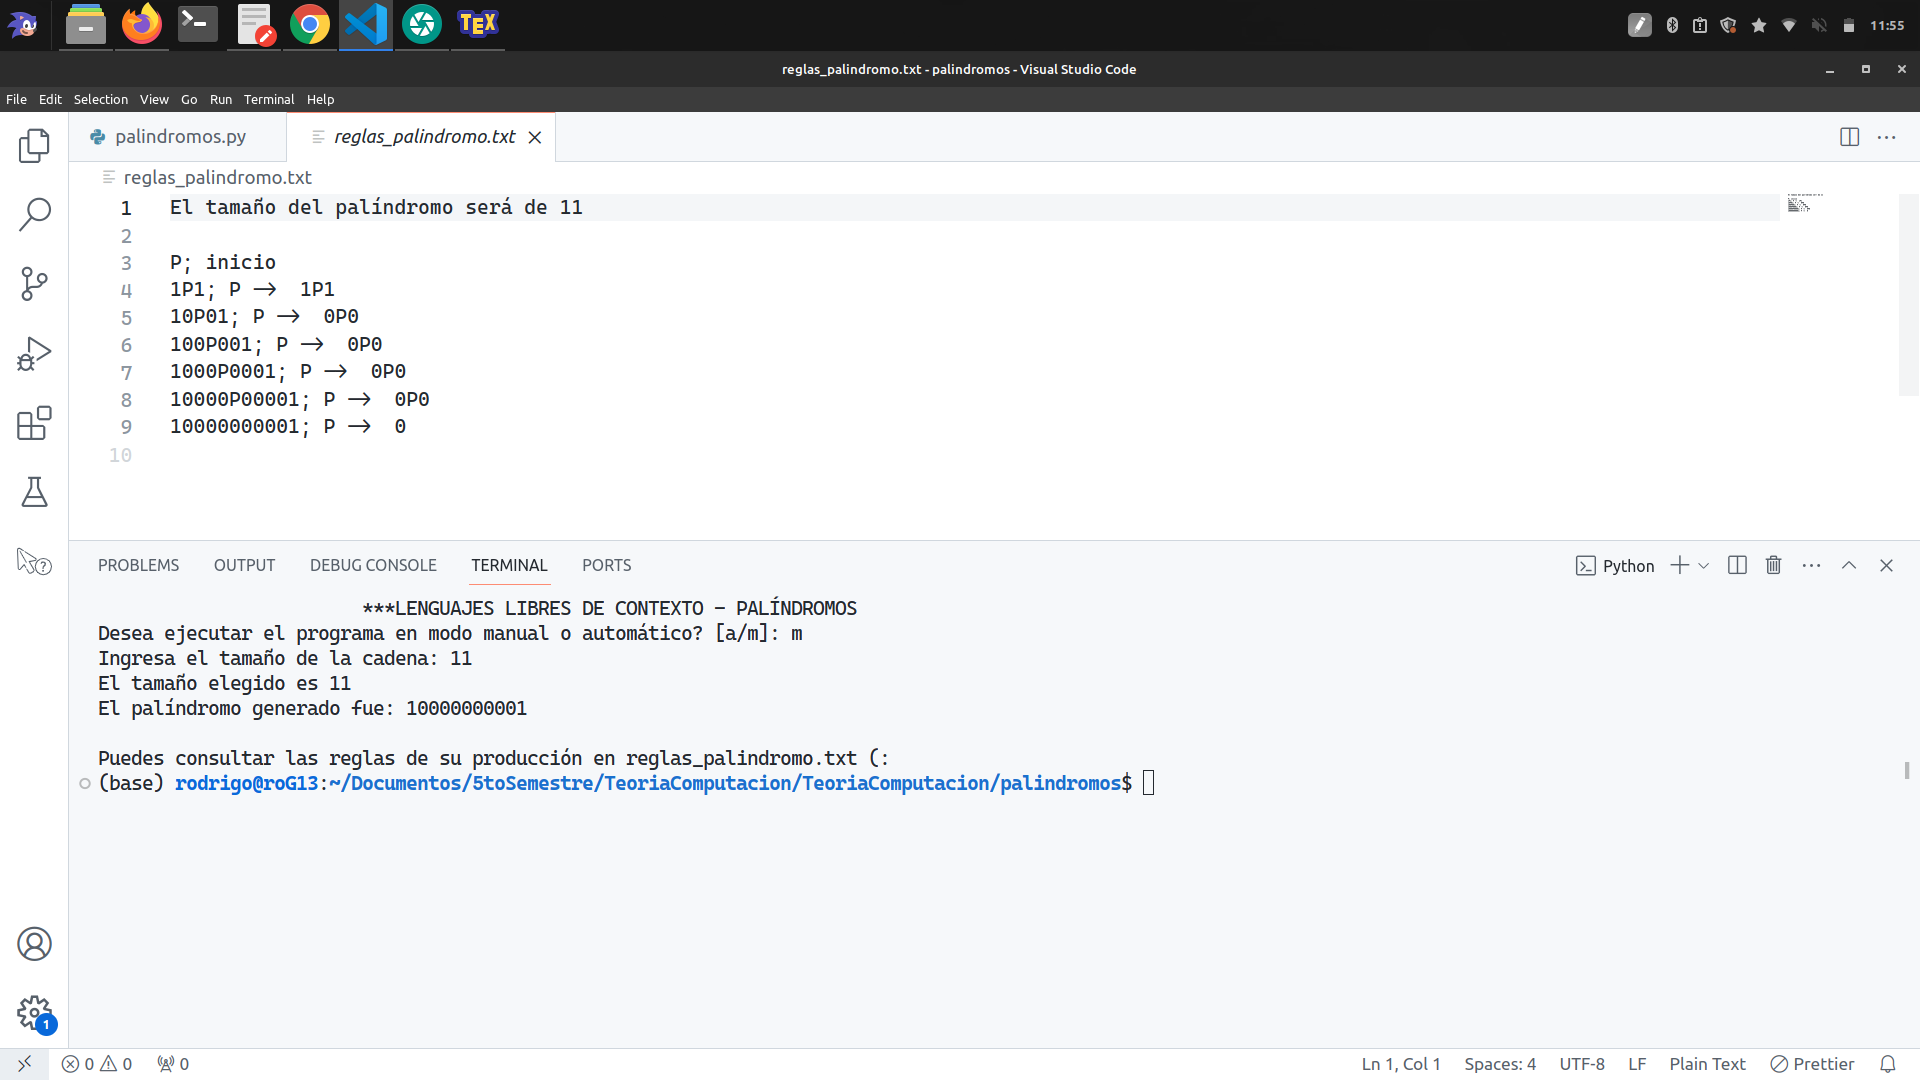
\includegraphics[width=0.8\textwidth]{arch2}
		\caption{Modo manual - Longitud impar - Archivo}
	\end{figure}
	
	\newpage
	
	\begin{figure}[h]
		\centering
		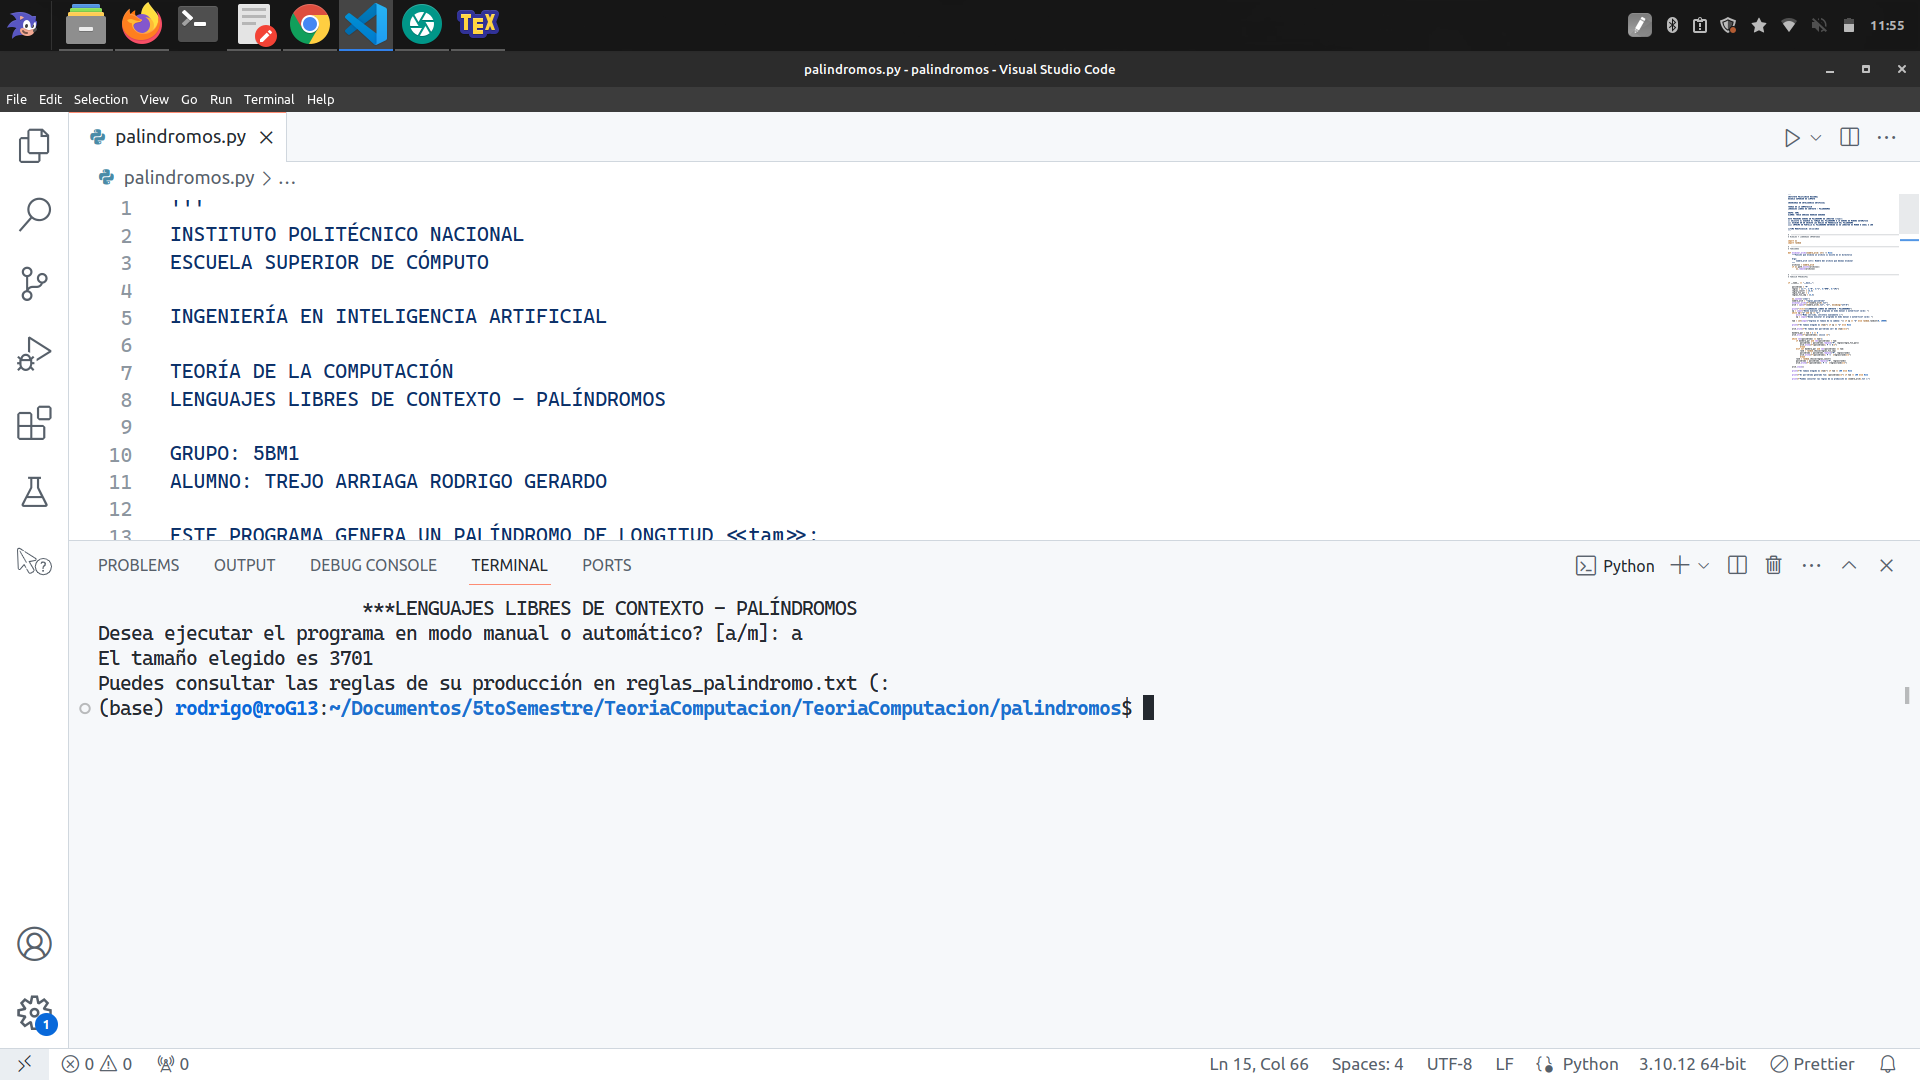
\includegraphics[width=0.8\textwidth]{auto}
		\caption{Modo automático}
	\end{figure}
	
	\begin{figure}[h]
		\centering
		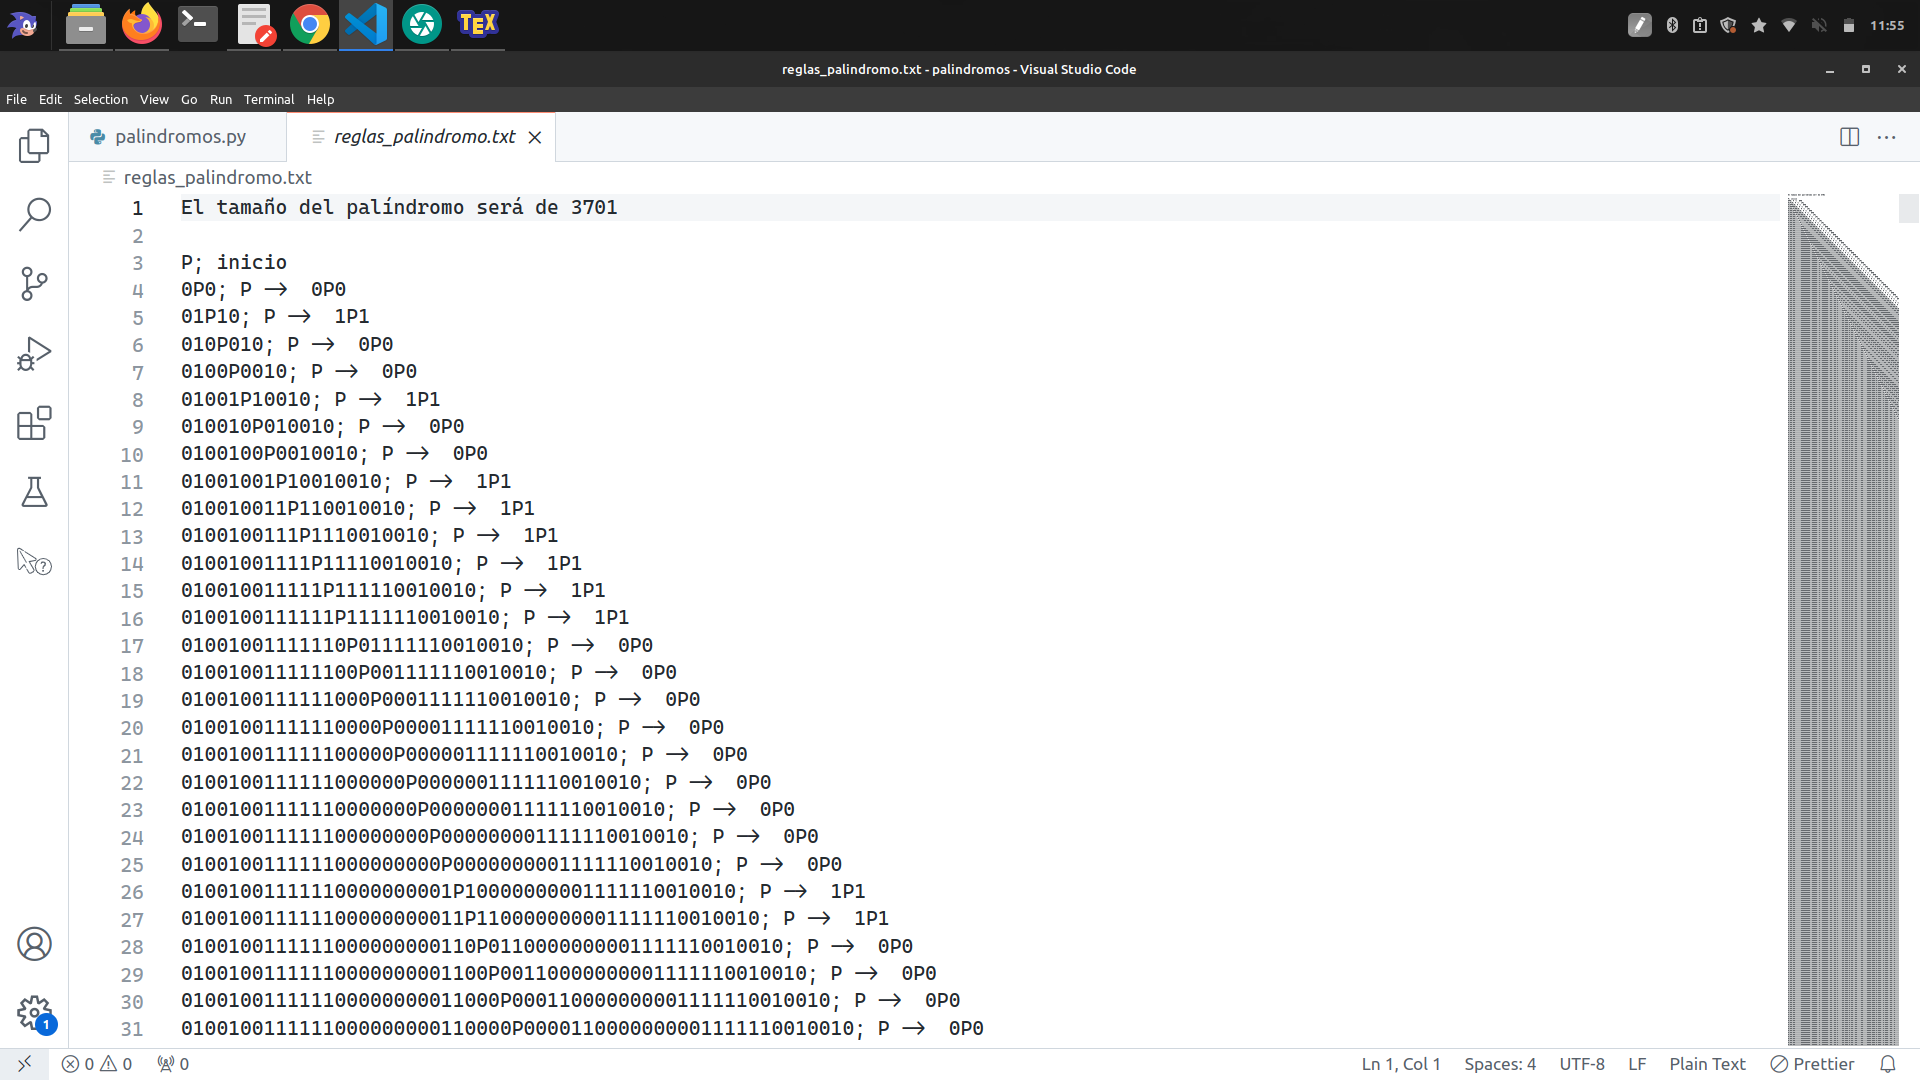
\includegraphics[width=0.8\textwidth]{arch3}
		\caption{Modo automático - Archivo}
	\end{figure}
	
	\newpage
	
	\begin{figure}[h]
		\centering
		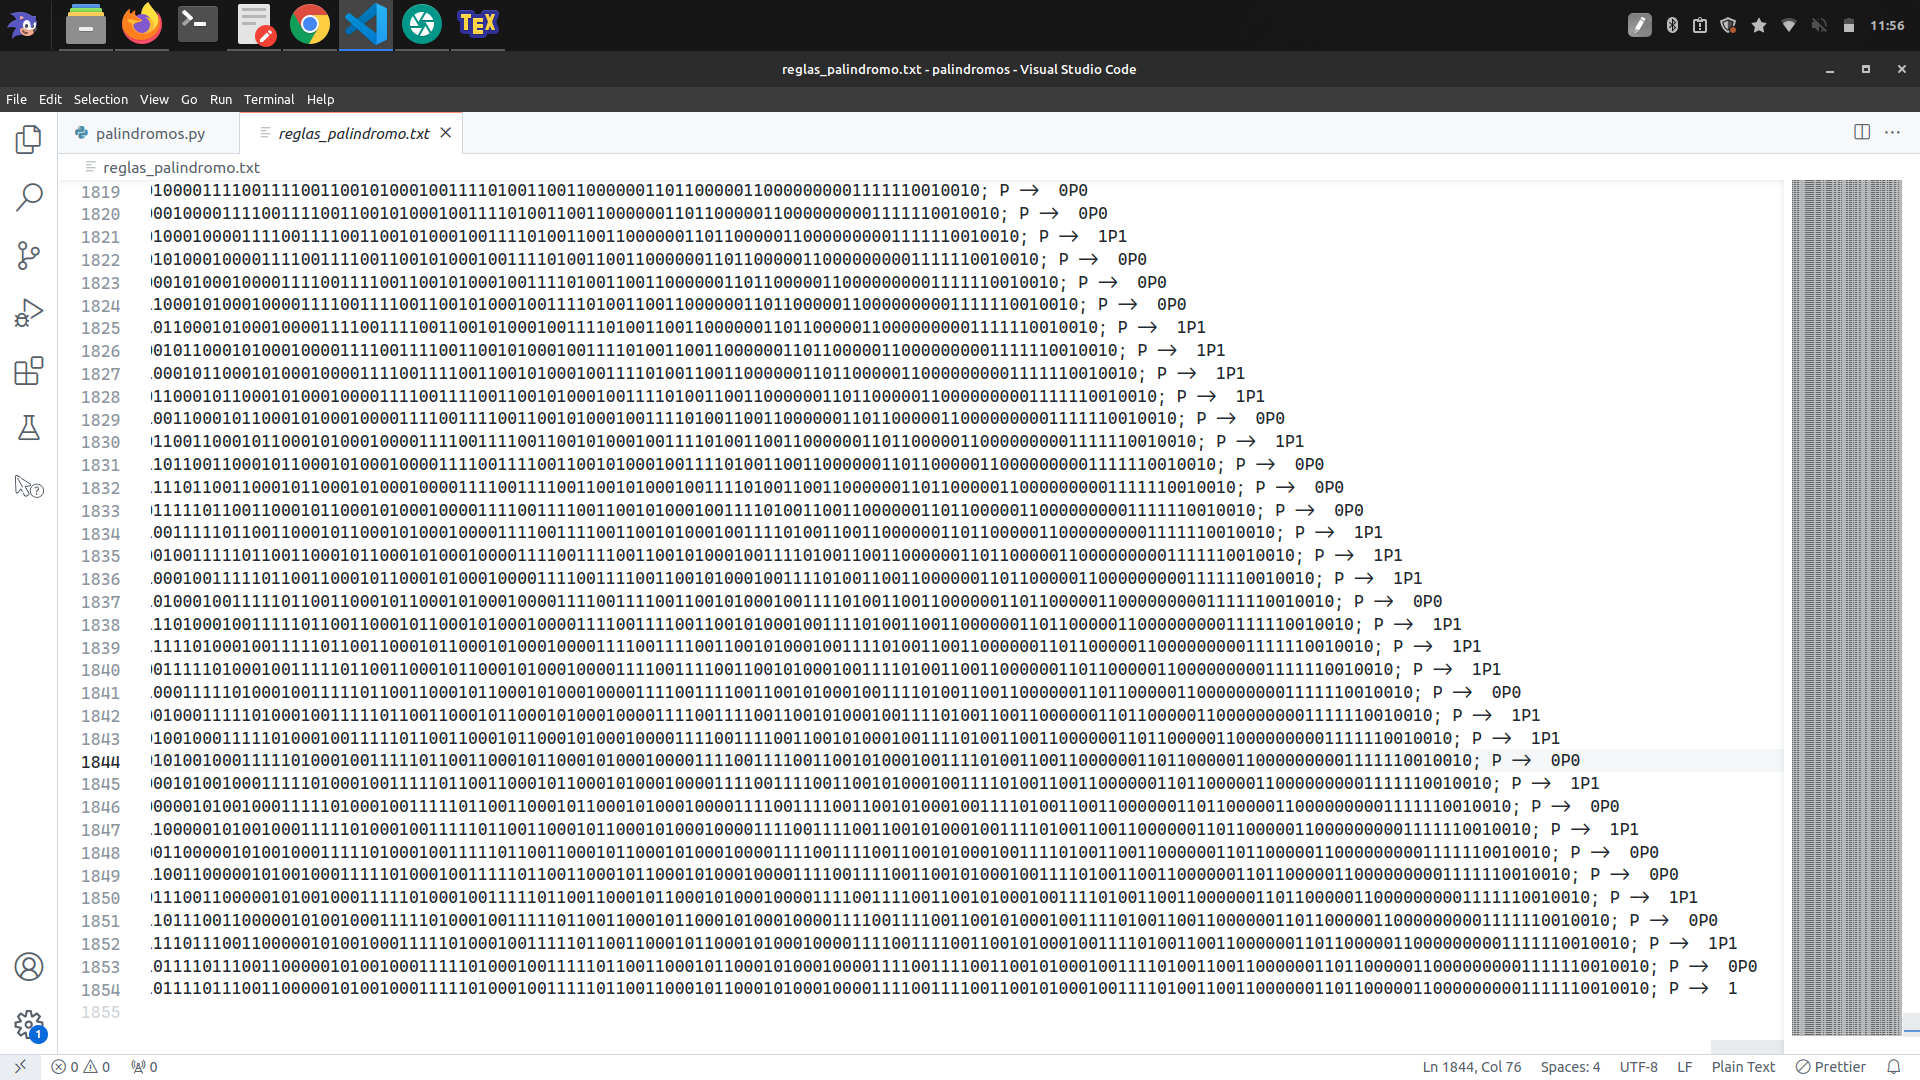
\includegraphics[width=0.8\textwidth]{arch4}
		\caption{Modo automático - Archivo}
	\end{figure}
	
	\newpage
	\section*{Conclusión}
	Esta práctica ha demostrado la eficacia de los lenguajes libres de contexto en la generación de estructuras simétricas como los palíndromos. Hemos explorado cómo una gramática simple puede ser utilizada para generar cadenas palindrómicas de forma sistemática y flexible, lo que demuestra la versatilidad de los lenguajes libres de contexto en la teoría de la computación.
	
	La implementación de un programa en Python para generar palíndromos binarios según la gramática definida ha proporcionado una comprensión práctica y aplicada de estos conceptos. Este enfoque nos ha permitido observar de primera mano la relación entre las reglas de producción de la gramática y la estructura final de los palíndromos generados.
	
	Además, la capacidad de generar palíndromos de manera aleatoria o con una longitud definida por el usuario muestra la flexibilidad y el potencial de este enfoque para diversas aplicaciones, desde el análisis de datos hasta la criptografía.
	
	Así, esta práctica ha reforzado la importancia de los lenguajes libres de contexto en el ámbito de la teoría de autómatas y la computación, destacando su utilidad para resolver problemas complejos de manera estructurada y eficiente.
	
	
	\section*{Bibliografía}
	
	
	[1] AcademiaLab. “Gramática libre de contexto \_ AcademiaLab”. Home | AcademiaLab. Accedido el 24 de diciembre de 2023. [En línea]. Disponible: https://academia-lab.com/enciclopedia/gramatica-libre-de-contexto/
	
	
	[2] Wikiwand. “Wikiwand - Gramática libre de contexto”. Wikiwand. Accedido el 24 de diciembre de 2023. [En línea]. Disponible: https://www.wikiwand.com/es/Gramática\_libre\_de\_contexto
	
	
	\newpage
	\section{Anexo - Código de Implementación}
	
	\begin{lstlisting}
		
		'''
		INSTITUTO POLITECNICO NACIONAL
		ESCUELA SUPERIOR DE COMPUTO
		
		INGENIERIA EN INTELIGENCIA ARTIFICIAL
		
		TEORIA DE LA COMPUTACION
		LENGUAJES LIBRES DE CONTEXTO - PALINDROMOS
		
		GRUPO: 5BM1
		ALUMNO: TREJO ARRIAGA RODRIGO GERARDO
		
		ESTE PROGRAMA GENERA UN PALINDROMO DE LONGITUD <<tam>>:
		i) SOLICITA AL USUARIO EL TAMANO DEL PALINDROMO O LO GENERA DE MANERA AUTOMATICA
		ii) ESCRIBE EN UN ARCHIVO LAS REGLAS DE PRODUCCION DEL PALINDROMO
		iii) IMPRIME EN PANTALLA EL PALINDROMO OBTENIDO SI SU LONGITUD ES MENOR O IGUAL A 100
		
		ULTIMA MODIFICACION: 24/12/2023
		'''
		
		#  ---------------------------------------------
		# MODULOS Y LIBRERIAS IMPORTADAS
		
		import os
		import random
		
		#  ---------------------------------------------
		# FUNCIONES
		
		def eliminar_archs(nombre_arch: str) -> None:
			"""Funcion que elimina un archivo si existe en el directorio
			
			Args:
			nombre_arch (str): Nombre del archivo que deseas eliminar
			"""
			archivo1 = nombre_arch
			if os.path.exists(archivo1):
			os.remove(archivo1)
		
		#  --------------------------------------------------
		# FUNCION PPRINCIPAL
		
		
		if __name__ == "__main__":
		
			palindromo = "P"
			reglas = {1:"", 2:"0", 3:"1", 4:"0P0", 5:"1P1"}
			reglas_constr = [4,5]
			regla_fin_par = 1
			reglas_fin_imp = [2,3]
			
			os.system('clear')
			nombre_arch = "reglas_palindromo"
			eliminar_archs(f"{nombre_arch}.txt")
			arch = open(f"{nombre_arch}.txt", "a+", encoding="utf-8")
			
			print("\t\t\t***LENGUAJES LIBRES DE CONTEXTO - PALINDROMOS")
			op = input("Desea ejecutar el programa en modo manual o automatico? [a/m]: ")
			while op!="a" and op != "m":
			print("Modo invalido, intentelo nuevamente ):")
			op = input("Desea ejecutar el programa en modo manual o automatico? [a/m]: ")
			
			tam = int(input("Ingresa el tamano de la cadena: ")) if op == "m" else random.randint(0, 10000)
			
			print(f"El tamano elegido es {tam}") if op == "a" else None
			
			arch.write(f"El tamano del palindromo sera de {tam}\n\n")
			
			bandera_par = tam % 2 == 0
			arch.write(f"{palindromo}; inicio \n")
			
			while len(palindromo) <= tam+1:
			if bandera_par and len(palindromo) > tam:
			palindromo = palindromo.replace("P", reglas[regla_fin_par])
			arch.write(f"{palindromo}; P -> e\n")
			break
			elif not bandera_par and len(palindromo) == tam:
			rand = random.choice(reglas_fin_imp)
			palindromo = palindromo.replace("P", reglas[rand])
			arch.write(f"{palindromo}; P ->  {reglas[rand]}\n")
			break
			rand = random.choice(reglas_constr)
			palindromo = palindromo.replace("P", reglas[rand])
			arch.write(f"{palindromo}; P ->  {reglas[rand]}\n")
			
			arch.close()
		
			print(f"El tamano elegido es {tam}") if tam <= 100 else None
			
			print(f"El palindromo generado fue: {palindromo}\n") if tam <= 100 else None
			
			print(f"Puedes consultar las reglas de su produccion en {nombre_arch}.txt (:")
		
		
	\end{lstlisting}
	
	
	
\end{document}